\documentclass[12pt]{article}
 
\usepackage[margin=1in]{geometry} 
\usepackage{mathtools}
\usepackage{bm}
\usepackage{subfig}
\usepackage{amssymb}
\usepackage{amsmath}
\usepackage{cleveref}
\usepackage{tikz}
\usetikzlibrary{bayesnet}
\usetikzlibrary{arrows}
\usepackage{graphicx}
\usetikzlibrary{positioning}

\setlength{\parskip}{1em}

\newenvironment{question}[2][Question]{\begin{trivlist}
\kern10pt
\item[\hskip \labelsep {\bfseries #1}\hskip \labelsep {\bfseries #2.}]}{\end{trivlist}}


\newcommand\TODO[1]{\textcolor{red}{#1}}
\newcommand\numberthis{\addtocounter{equation}{1}\tag{\theequation}}
\begin{document}
 
% --------------------------------------------------------------
%                         Start here
% --------------------------------------------------------------
 
%\renewcommand{\qedsymbol}{\filledbox}
 
\title{DD2434 Machine Learning, Advanced Course Assignment 1}
\author{Lin Chun Hung, chlin3@kth.se} 
 
\maketitle


% Question 1
\begin{question}{1}
The Gaussian form of likelihood is a sensible choice.
We have assumed that the observed values $\bf{t}_i$ differ from the function values
or the mapped input values $f(\bf{x}_i)$ by additive Gaussian noise.
\begin{align*}
  \mathbf{t}_i = f(\mathbf{x}_i) + \bm{\epsilon}
\end{align*}
The noise is gaussian:
\begin{align*}
  \bm{\epsilon} \sim \mathcal{N}(\mathbf{0}, \sigma^2\mathbf{I})
\end{align*}
And each components the noise is:
\begin{align*}
  \epsilon_j \sim \mathcal{N}(0, \sigma_j^2)
\end{align*}

Combine these two assumptions, we have the Gaussian form likelihood.

The assumption of gaussian noise is also sensible.
Consider that we draw a lot of samples from the population.
If we consider the noise of each observation as an random variable, then the sum
(or the average) of noise will be a random variable following a normal distribution 
by the central limit theorem. Therefore, we can consider the noise across 
all samples as an independent and identically distributed random variable 
following a normal distribution.

The unbias noise assumption is correct since if the noise is biased we can move the
bias term to the function $f(\bf{x}_i)$.

With the assumption that features are uncorrelated, we choose the spherical
covariance matrix for the likelihood.
\end{question}
% End question 2



% Question 2
\begin{question}{2}
Consider the general product rule of probability:
$$\mathrm {P} \left(\bigcap _{k=1}^{n}A_{k}\right)=
  \prod _{k=1}^{n}\mathrm {P} \left(A_{k}\,{\Bigg |}\,\bigcap _{j=1}^{k-1}A_{j}\right)$$

Therefore the likelihood would be:
$$ 
  p(\mathbf{T}\mid f,\mathbf{X}) =
  \prod _{i=1}^{N}p(\mathbf{t}_i \mid \mathbf{t}_{i-1},...,\mathbf{t}_{1},
  f,\mathbf{X})
$$

\end{question} 
% End question 2


% Question 3 
\begin{question}{3}

$$ 
  p(\mathbf{T}\mid \mathbf{X},\mathbf{W}) =
  \prod _{i=1}^{N}\mathcal{N}(\mathbf{W}\mathbf{x}_i, \sigma^2\mathbf{I})
$$

\end{question}
% End question 3

% Question 4
\begin{question}{4}
The choice of the prior distribution reflects the choice of regularizer. 
Chossing $L_1$ norm as regularizer is known as the lasso (least absolute shrinkage and selection operator).
The regularizer will force some weighting coefficients $w_j$ to be zero, given 
a proper choice of model parameter $\tau$. It plays the role of feature selection
since those zero weighting coefficients indicate that the corresponding features
are irrelvant to the output.

The penalization term or the negative log-prior:
\begin{align*}
  \frac{\lambda}{2} \left \|\textbf{vec}(\bf{W} - \bf{W}_0)\right \|_{q}  
\end{align*}
If $q = 1$, that is the absolute-value norm.
If $q = 2$, that is the euclidean norm.

In figure \ref{fig:Q4-min-reg},
we can see that in the corresponding minimization problem (i.e. least sqare problem).
The regularization term acts as a constrain in the minimization problem.

In the right head side of the figure, it is a minimization problem using $L_1$
regularization term.
If using $L_1$ norm, the minimization result $\mathbf{w}^{*}$ is forced to lay on 
the $w_2$ axis and the parameter $w_1$ of $\mathbf{w}^{*}$ becomes zero and which
can be understood as feature selection. In the figure, the contrains is a square
shape contour.

If using $L_2$ norm, the contrain is a circle as the form of the regularization 
term.


\begin{figure}[h!]
  \centering
  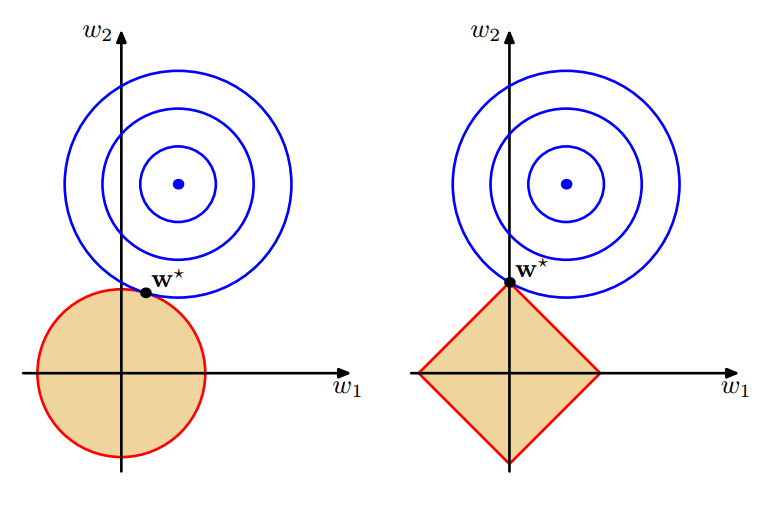
\includegraphics[width=0.5\linewidth]{q4_regular.png}
  \caption{Plot contours of the error minimization problems}
  \label{fig:Q4-min-reg}
\end{figure}

\end{question}
% End question 4



% Question 5
\begin{question}{5}
Consider the regression equation in general:
$$\textbf{T} = \textbf{WX} + \textbf{ErrorMatrix} $$
Therefore, the likelihood in terms of matrix normal distribution is:
\begin{align*}
p(\bf{T}\mid \bf{X}, \bf{W}) &= 
  \mathcal{MN}_{D \times N}(\bf{WX}, \bf{I}, \sigma^2 \bf{I}) \\ 
  &= \mathcal{N}_{DN}(\bf{vec}(\bf{WX}), \sigma^2 \bf{I})
\end{align*}
The prior is:
\begin{align*}
p(\bf{W}) &= 
  \mathcal{MN}_{D \times q}(\textbf{W}_0, \bf{I}, \tau^2 \bf{I}) \\
  &= \mathcal{N}_{Dq}(\textbf{vec}(\textbf{W}_0), \tau^2 \bf{I})
\end{align*}

Due to the choice of a conjugate Gaussian prior distribution, the posterior will 
also be Gaussian:
$$
p(\textbf{W}\mid \textbf{X}, \textbf{T}) =
  \mathcal{N}_{Dq}(\textbf{vec}(\textbf{W}_{p0}), \bm{\Sigma}_{p0} )
$$

To calculate the mean and covariance of the posterior over the parameters,
Consider the equation 7 in the question with respect to the parameters $\textbf{W}$
 and compare the quadratic and linear terms of the exponents in both sides:
\begin{align*}
  p(\textbf{W}\mid \textbf{X}, \textbf{T}) =&
  \frac{1}{Z}p(\textbf{T}\mid \textbf{X}, \textbf{W})p(\textbf{W})  \\
  \ln p(\textbf{W}\mid \textbf{X}, \textbf{T}) =&
  \ln p(\textbf{T}\mid \textbf{X}, \textbf{W}) + \ln p(\textbf{W}) + \text{Const.} \\
\end{align*}
\begin{align*}
  LHS =& -\frac12[\textbf{vec}(\textbf{W}) - \textbf{vec}(\textbf{W}_{p0)}]^T
          \bm{\Sigma}_{p0}^{-1}[\textbf{vec}(\textbf{W})-\textbf{vec}(\textbf{W}_{p0})] \\
  RHS =& -\frac{1}{2\sigma^2}[\textbf{vec}(\textbf{T}) - \textbf{vec}(\textbf{WX})]^T
                             [\textbf{vec}(\textbf{T}) - \textbf{vec}(\textbf{WX})] \\
       &-\frac{1}{2\tau^2}[\textbf{vec}(\textbf{W}) - \textbf{vec}(\textbf{W}_0)]^T
                          [\textbf{vec}(\textbf{W}) - \textbf{vec}(\textbf{W}_0)] \\
       &+\text{Const.} \numberthis \label{eq:Q5-loglike-RHS}
\end{align*}
We ignore those terms which are not functions of $\mathbf{W}$ and say they are constants.

Consider the quadratic terms on both sides:
\begin{equation} \label{eq:q5-covar}
  \begin{aligned}[b]
    -\frac12\textbf{vec}(\textbf{W})^T\bm{\Sigma}_{p0}^{-1}\textbf{vec}(\textbf{W})
    =& -\frac{1}{2\sigma^2}\textbf{vec}(\textbf{WX})^T\textbf{vec}(\textbf{WX})
    -\frac{1}{2\tau^2}\textbf{vec}(\textbf{W})^T\textbf{vec}(\textbf{W}) \\
    -\frac12\textbf{vec}(\textbf{W})^T\bm{\Sigma}_{p0}^{-1}\textbf{vec}(\textbf{W})
    =& -\frac{1}{2\sigma^2}\textbf{vec}(\textbf{W})^T(\mathbf{X}^T \otimes \mathbf{I}_D)^T
    (\mathbf{X}^T \otimes \mathbf{I}_D)\textbf{vec}(\textbf{W}) \\
    & -\frac{1}{2\tau^2}\textbf{vec}(\textbf{W})^T\textbf{vec}(\textbf{W}) \\
    -\frac12\bm{\Sigma}_{p0}^{-1} =&
    -\frac{1}{2\sigma^2}(\mathbf{X} \otimes \mathbf{I}_D)(\mathbf{X}^T \otimes \mathbf{I}_D) 
    -\frac{1}{2\tau^2} \mathbf{I}_{Dq}\\
    \bm{\Sigma}_{p0}^{-1} =& \hspace{5mm} 
    \frac{1}{\sigma^2}(\mathbf{X}\mathbf{X}^T)\otimes \mathbf{I}_D +\frac{1}{\tau^2}\mathbf{I}_{Dq}
  \end{aligned}
\end{equation}

Consider the linear terms on both sides:  
\begin{align*}
    \textbf{vec}(\textbf{W})^T\bm{\Sigma}_{p0}^{-1}\textbf{vec}(\textbf{W}_{p0})
    =& \hspace{1mm} 
       \frac{1}{\sigma^2}\textbf{vec}(\textbf{WX})^T\textbf{vec}(\textbf{T}) 
     + \frac{1}{\tau^2}\textbf{vec}(\textbf{W})^T\textbf{vec}(\textbf{W}_0)\\
    \textbf{vec}(\textbf{W})^T\bm{\Sigma}_{p0}^{-1}\textbf{vec}(\textbf{W}_{p0})
    =& \hspace{1mm} 
       \frac{1}{\sigma^2}\textbf{vec}(\textbf{W})^T(\mathbf{X}\otimes\mathbf{I}_D)
       \textbf{vec}(\textbf{T}) 
     + \frac{1}{\tau^2}\textbf{vec}(\textbf{W})^T\textbf{vec}(\textbf{W}_0)\\
    \textbf{vec}(\textbf{W}_{p0}) =& \hspace{1mm} 
       \bm{\Sigma}_{p0}[\frac{1}{\sigma^2}(\mathbf{X}\otimes\mathbf{I}_D)
       \textbf{vec}(\textbf{T}) + \frac{1}{\tau^2}\textbf{vec}(\textbf{W}_0)] \\
\end{align*}
\begin{equation} \label{eq:q5-mean}
    \textbf{vec}(\textbf{W}_{p0}) =
    [\frac{1}{\sigma^2}(\mathbf{X}\mathbf{X}^T)\otimes \mathbf{I}_D +\frac{1}{\tau^2}\mathbf{I}_{Dq}]^{-1}
       [\frac{1}{\sigma^2}(\mathbf{X}\otimes\mathbf{I}_D)
       \textbf{vec}(\textbf{T}) + \frac{1}{\tau^2}\textbf{vec}(\textbf{W}_0)]
\end{equation}

Consider the equation \eqref{eq:Q5-loglike-RHS}, it is the right hand side of the
log posterior. If we maximize it, the first term corresponds to minimize the
least square term. And the second term can be viewed as the regularization term.
Therefore, the first term of the log posterior is related to minimizing 
the least square error of the linear regression problem.

Consider an infinitely broad prior, which means $\tau \to \infty$, reduces the 
mean and covariance of the posterior to the mean and covariance of the likelihood
estimated under maximum likelihood approach.

The constant $Z$ plays no role in the calculation since only the quadratic and linear
 terms are considered.
% Subsitute back \eqref{eq:q5-covar} and \eqref{eq:q5-mean} into the posterior

\end{question}
% End question 5

% Question 6
\begin{question}{6}
% \begin{align*}
%   p(f\mid X,\theta) = N(0, k(X, X))  % TODO: fix this equation
% \end{align*}
  The prior distribution over functions expresses our beliefs and knowledge about
how the function looks like before we consider the data.

We choose the mean function as zero
since we have forced the data to have zero-mean. We can choose a non-zero mean
function of the Gaussian process. Indeed, we can use a fixed mean function, but
the result is trivial that we can obtain the predictive mean function by adding 
the mean-removal result to the fixed mean function.
(Rasmussen, C. E., 2004, page 27)

The covariance of the prior, is the covariance
function controlled by the hyperparameter $\bm{\theta}$. The covariance function
tells that if two input points are similar, then the output should be similar as
well. The specification of the covariance function indicates a distribution over 
functions. To visualize it, we can draw some smaples from the distribution of 
function evaluated at some test input points.

Moreover, if we consider the marginal likelihood:
\begin{align*}
  p(\mathbf{T}\mid\mathbf{X}, \bm{\theta}) 
    &= \int p(\mathbf{T}\mid f)p(f\mid \mathbf{X}, \bm{\theta})df
\end{align*}
It means we consider all possible functions and average data likelihood over on those functions.
It also means we aggregate the information from prior and likelihood to estimate the
probability of evidence.

If we draw some samples from the predictive posterior, we can find that the 
covariance of the prior controls how to predict the unobserved points in bayesian
view.

%TODO: Fix this figure, use python to replot it
\begin{figure}[h!]
  \centering
  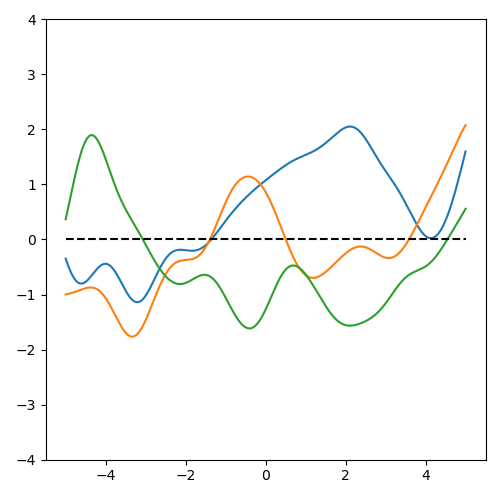
\includegraphics[width=0.5\linewidth]{fig/Q6-prior.png}
  \caption{Sample functions sampled from the prior}
\end{figure}
\begin{figure}[h!]
  \centering
  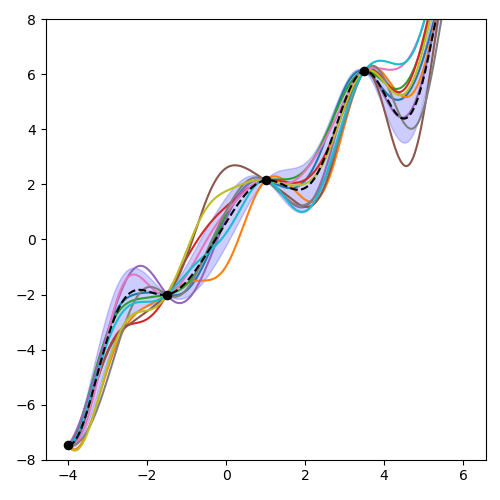
\includegraphics[width=0.5\linewidth]{fig/Q6-post-l110.png}
  \caption{Sample predictive functions, predictive mean, and predictive covariance}
\end{figure}
\end{question}

% Question 7
\begin{question}{7}
  \begin{figure}[h!]
    \centering
    \tikz{
      % nodes
      \node[latent] (f) {$f$};
      \node[latent,above=of f,xshift=1cm] (X) {$\mathbf{X}$}; %
      \node[latent,above=of f,xshift=-1cm] (theta) {$\bm{\theta}$}; %
      \node[latent,below=of f,xshift=0cm] (T) {$\mathbf{T}$}; %
      % edges
      \edge {theta,X} {f}  
      \edge {f} {T}  
    }
  \caption{The graphical model showing the assumption of the joint likelihood}
  \label{fig:Q7-graphs}
  \end{figure}
  \begin{align*}
    p(\mathbf{T}, \mathbf{X}, f, \bm{\theta}) 
      = p(\mathbf{T}\mid f)p(f \mid \mathbf{X},\bm{\theta})
      p(\mathbf{X})p(\bm{\theta}) 
  \end{align*}

The graphical model is shown in figure \ref{fig:Q7-graphs}
\end{question}

\begin{question}{8}
\begin{align*}
  p(\mathbf{T} \mid \mathbf{X}, \bm{\theta}) = \int p(\mathbf{T}\mid f)p(f) df
\end{align*}

The marginalisation connects the prior and the likelihood of the data. The
integral is an weighted average averaging the likelihood of the data with the prior
as weighting.

The uncertainties of the data and the prior are combined or added up into the 
uncertainty of the marginalisation. The covariance of the marginalisation is
$k(\mathbf{X},\mathbf{X}) + \sigma^2\mathbf{I}$. The first term comes from the
uncertainty of the prior. 
The second term comes from the uncertainty of data likelihood.


The hyperparameters $\bm{\theta}$ still condition on the part of covariance of the 
 marginalisation from the prior. That part of covariance is the kernel function.
\end{question}

\begin{question}{9}
We set the prior distribution as:
  \begin{align*}
    p(\mathbf{W}) = 
      \mathcal{N}(
        \begin{bmatrix}
          0\\ 
          0
        \end{bmatrix},
        \begin{bmatrix}
          2 & 0\\ 
          0 & 2
        \end{bmatrix}
      )
  \end{align*}
And the figure \ref{fig:Q9-prior} shows the prior distribution over $\mathbf{W}$
\begin{figure}[h!]
  \centering
  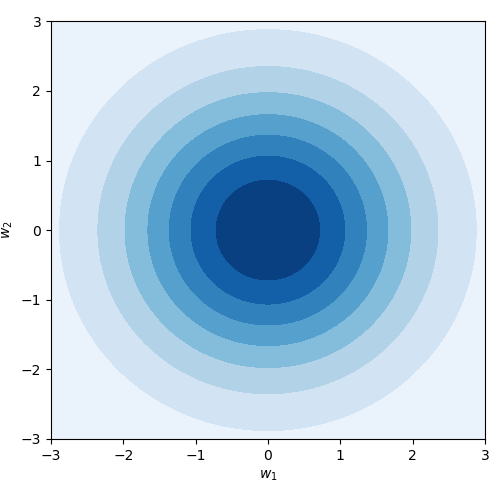
\includegraphics[width=0.5\linewidth]{fig/Q9-prior.png}
  \caption{Prior distribution over $\mathbf{W}$}
  \label{fig:Q9-prior}
\end{figure}

\begin{figure}[h!]
  \subfloat[Posterior distribution over $\mathbf{W}$]{%
  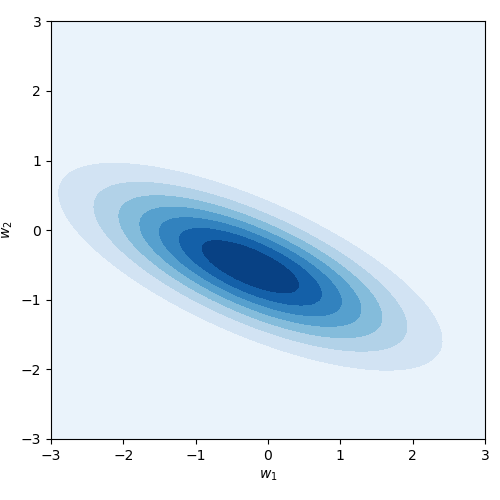
\includegraphics[width=0.45\textwidth]{fig/Q9-post-s3-n1.png}
  }
  \hfill
  \subfloat[Functions with the parameters sampled from the posterior]{%
  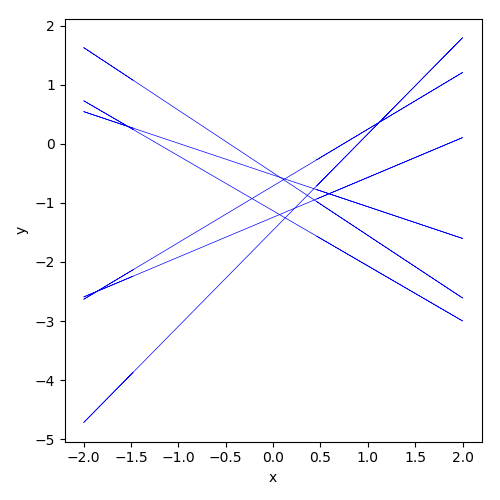
\includegraphics[width=0.45\textwidth]{fig/Q9-fun-s3-n1.png}
  }
  \caption{The posterior and the resulting functions with 1 data point, $\sigma = 0.3$}
\end{figure}

\begin{figure}[h!]
  \subfloat[Posterior distribution over $\mathbf{W}$]{%
  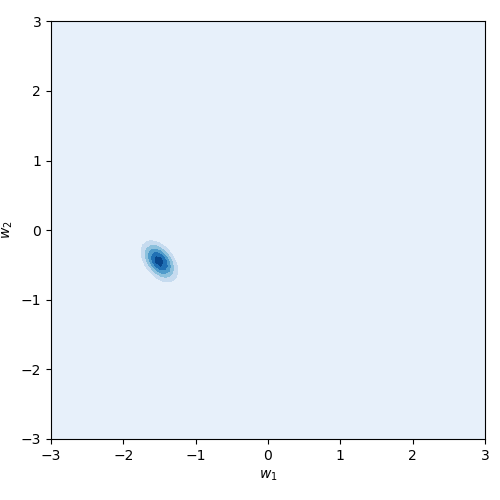
\includegraphics[width=0.45\textwidth]{fig/Q9-post-s1-n5.png}
  }
  \hfill
  \subfloat[Functions with the parameters sampled from the posterior]{%
  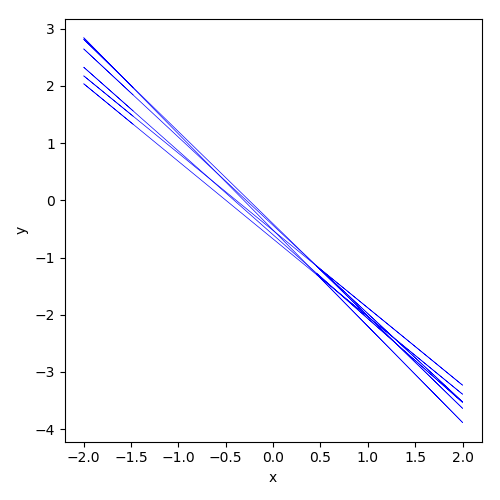
\includegraphics[width=0.45\textwidth]{fig/Q9-fun-s1-n5.png}
  }
  \caption{The posterior and the resulting functions with 5 data points, $\sigma = 0.1$}
\end{figure}

\begin{figure}[h!]
  \subfloat[Posterior distribution over $\mathbf{W}$]{%
  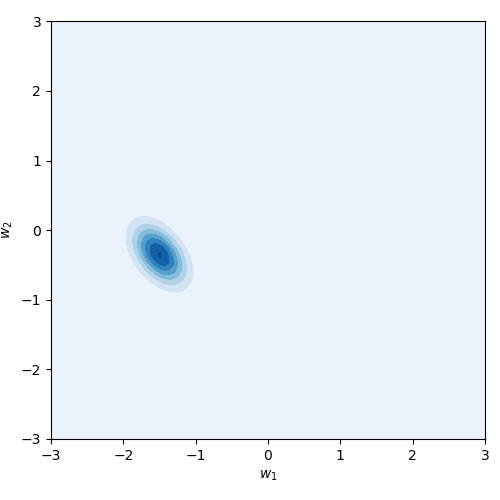
\includegraphics[width=0.45\textwidth]{fig/Q9-post-s3-n5.png}
  }
  \hfill
  \subfloat[Functions with the parameters sampled from the posterior]{%
  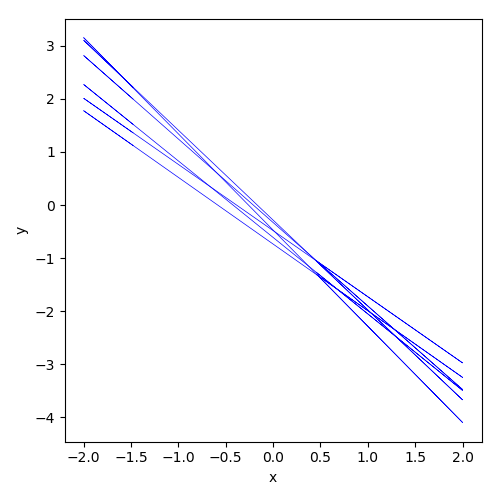
\includegraphics[width=0.45\textwidth]{fig/Q9-fun-s3-n5.png}
  }
  \caption{The posterior and the resulting functions with 5 data points, $\sigma = 0.3$}
\end{figure}

When more data observed, the posterior become concentrated over the parameter space.
In general, we can say that the posterior receive more information about data.
Therefore, the posterior can have more confident to tell what is the underlying 
parameter behind the data. On the other hand, the posterior gaussian covariance
could be expressed as 
$(\frac{1}{\sigma^2}\mathbf{X}\mathbf{X}^T + \frac{1}{\tau^2}\mathbf{I})^{-1}$.
The more data observed, the determinant of $\mathbf{X}\mathbf{X}^T$ will be 
larger and the determinant of covariance matrix will be smaller.

\begin{figure}[h!]
  \subfloat[Posterior distribution over $\mathbf{W}$]{%
  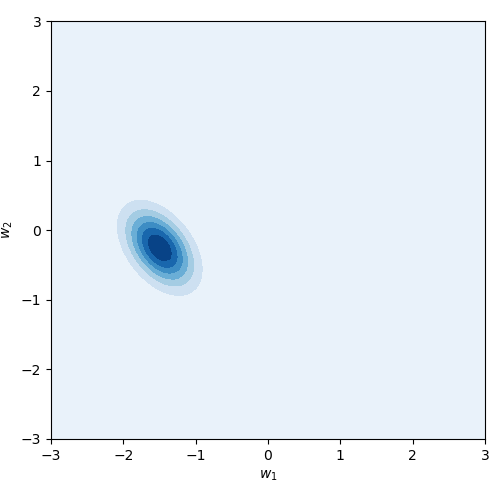
\includegraphics[width=0.45\textwidth]{fig/Q9-post-s5-n5.png}
  }
  \hfill
  \subfloat[Functions with the parameters sampled from the posterior]{%
  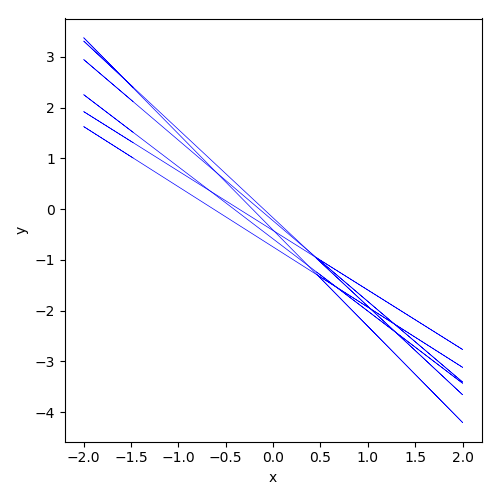
\includegraphics[width=0.45\textwidth]{fig/Q9-fun-s5-n5.png}
  }
  \caption{The posterior and the resulting functions with 5 data points, $\sigma = 0.5$}
\end{figure}

\begin{figure}[h!]
  \subfloat[Posterior distribution over $\mathbf{W}$]{%
  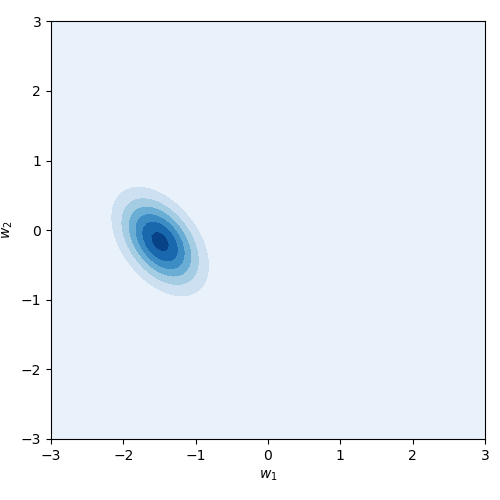
\includegraphics[width=0.45\textwidth]{fig/Q9-post-s7-n5.png}
  }
  \hfill
  \subfloat[Functions with the parameters sampled from the posterior]{%
  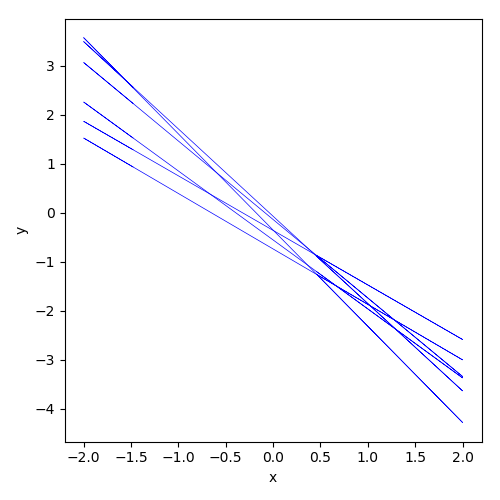
\includegraphics[width=0.45\textwidth]{fig/Q9-fun-s7-n5.png}
  }
  \caption{The posterior and the resulting functions with 5 data points, $\sigma = 0.7$}
\end{figure}

Consider the noise with different values of $\sigma$, the spreading of the 
probability distribution of posterior over $\mathbf{W}$ increases as the sigma
value increases. As the uncertainty of posterior increases, the models or the 
resulting functions variate more.
\end{question}

\begin{question}{10}
Consider a Gaussian process:
  \begin{align*}
    f(\mathbf{x}) \sim \mathcal{GP}(\mathbf{0}, k(\mathbf{X}, \mathbf{X'}))
  \end{align*}
The kernel function is:
\begin{align*}
  k(\mathbf{x}_i, \mathbf{x}_j) = \sigma^2_f \exp(-\frac{||\mathbf{x}_i - \mathbf{x}_j||^2}{l^2})
\end{align*}
We choose $\sigma^2_f = 1$ for the sake of convenience.

\begin{figure}[h!]
  \subfloat[$l = 0.05$]{%
  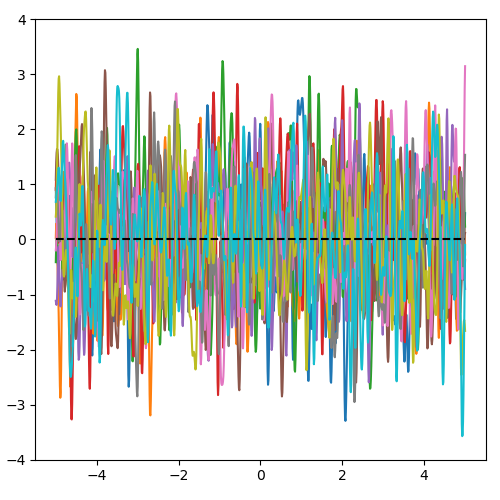
\includegraphics[width=0.4\textwidth]{fig/Q10-l005.png}
  }
  \hfill
  \subfloat[$l = 0.5$]{%
  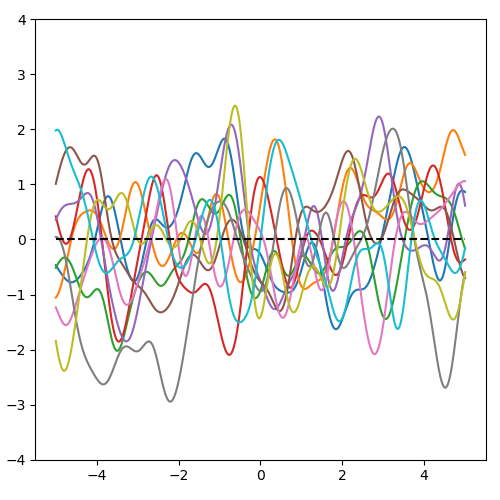
\includegraphics[width=0.4\textwidth]{fig/Q10-l050.png}
  }
  \vskip\baselineskip
  \subfloat[$l = 1.0$]{%
  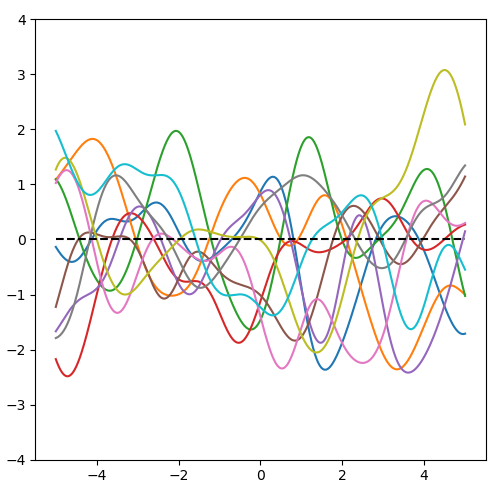
\includegraphics[width=0.4\textwidth]{fig/Q10-l100.png}
  }
  \hfill
  \subfloat[$l = 10.0$]{%
  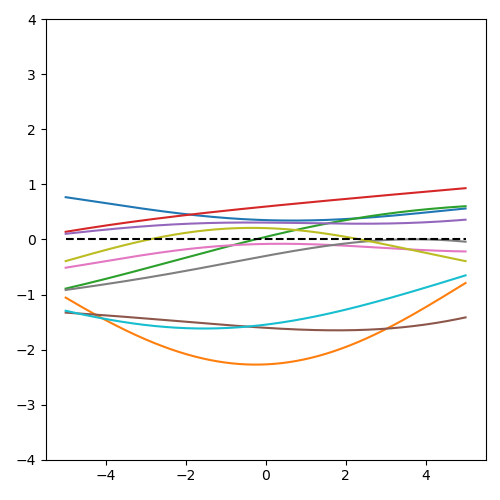
\includegraphics[width=0.4\textwidth]{fig/Q10-l1000.png}
  }
  \caption{Samples from priors with different length scales}
\end{figure}

For the case $l = 0.05$, the correlations among points tend to zero. Therefore,
the prior behaves as white noise.

When the length scale increases, the correlation of each pair of points increases.
If the correlation is strong enough, each sample function will become a straight line.
Therefore, as the correlation increases, the fluctuation of the sample functions decreases.
\end{question}

\begin{question}{11}
The posterior and the prior are the same if we do not have any observed data.
The posterior can be written as $p(f\mid \mathbf{t})$ which means given certain data
$\mathbf{t}$ the probability of a random variable $f$. 
If there is no given data, then obviously
the probability of the random variable $f$ is $p(f)$ which is the prior.

Here, we consider the sample observations are noise free.
And the prediction posterior distribution can be written as:
\begin{align*}
  \mathbf{f}_{*} \mid \mathbf{X}_{*}, \mathbf{X}, \mathbf{t} \sim \mathcal{N}(&
    K(\mathbf{X}_*, \mathbf{X})K(\mathbf{X}, \mathbf{X})^{-1}\mathbf{t}, \\
    &K(\mathbf{X}_*, \mathbf{X}_*) 
      - K(\mathbf{X}_*, \mathbf{X})K(\mathbf{X}, \mathbf{X})^{-1}K(\mathbf{X}, \mathbf{X}_*),
  )
\end{align*}
where $\mathbf{X}_*$ is the test input and $\mathbf{f}_{*}$ is the corresponding output.

Sample functions, predictive mean and variance of the posterior are shown in 
figure \ref{fig:Q11-predict-post}. The black dash lines are the predictive mean
functions. The blue shadows are the range from $\mu - \sigma$ to $\mu + \sigma$.

The results are desirable. For $l = 0.05$, the prior indicates that each point 
are almost uncorrelated. The mean function shows this point. For $l = 0.1$ and $l = 1.0$,
we can see that the mean function becomes less fluctuating. For $l = 10$, sample
noise ($\sigma^2 = 0.1$) is added to avoid the invalid inverse of the gram matrix
$K(\mathbf{X}, \mathbf{X})$ to be zero. 
The sample functions alters a bit compared to the prior since the strong asumption
on the correlation of points. In other words, the prior indicate that it is a 
restrictive model and therefore data can not alter the model too much.

\begin{figure}[h!]
  \subfloat[$l = 0.05$]{%
  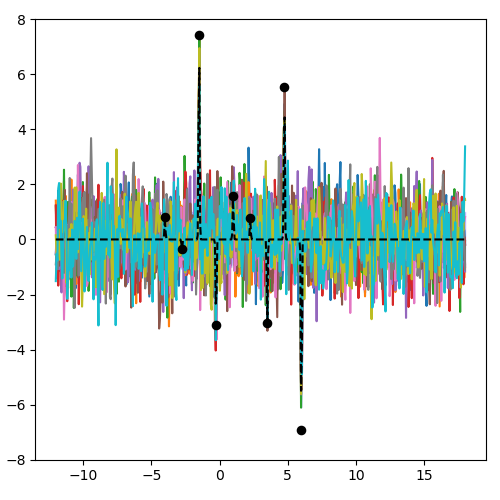
\includegraphics[width=0.4\textwidth]{fig/Q10-post-l005.png}
  }
  \hfill
  \subfloat[$l = 0.5$]{%
  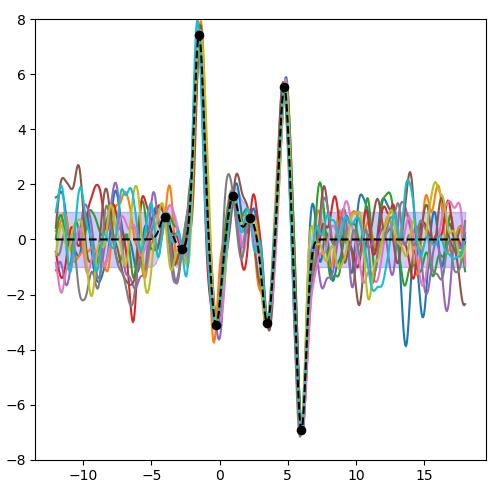
\includegraphics[width=0.4\textwidth]{fig/Q10-post-l050.png}
  }
  \vskip\baselineskip
  \subfloat[$l = 1.0$]{%
  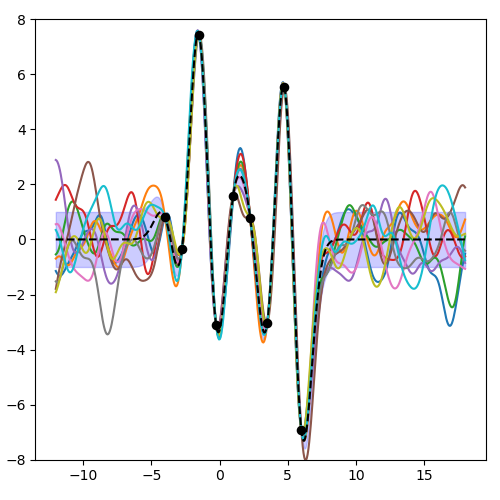
\includegraphics[width=0.4\textwidth]{fig/Q10-post-l100.png}
  }
  \hfill
  \subfloat[$l = 10.0$]{%
  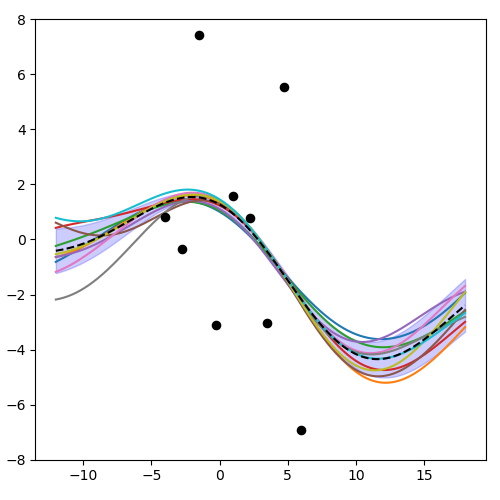
\includegraphics[width=0.4\textwidth]{fig/Q10-post-l1000.png}
  }
  \caption{Sample functions, mean and variance of the prediction posterior with different length scales}
  \label{fig:Q11-predict-post}
\end{figure}

Consider the covariance matrix in the prior is:
\begin{align*}
  k(\mathbf{x}_i, \mathbf{x}_j) + \sigma^2\delta_{ij}
\end{align*}
It is equivalent to considing the sample noise. The predictive posterior will
move towards to the prior since the likelihood of data becomes less informative.

Consider the noise is Gaussian with zero-mean and the variance is 4 (because $t_i$ is 1-d).
The results are shown in figure \ref{fig:Q11-predict-post-noise4}.
\begin{figure}[h!]
  \subfloat[$l = 0.05$]{%
  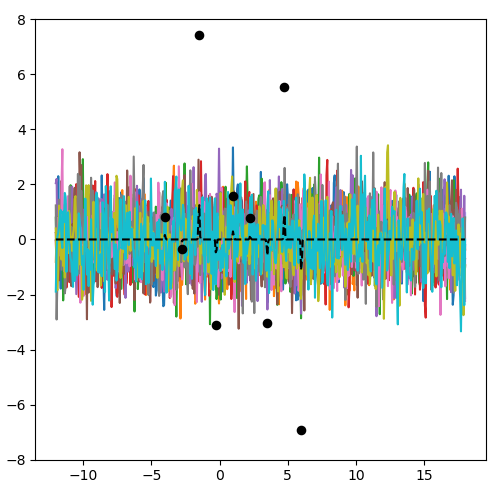
\includegraphics[width=0.4\textwidth]{fig/Q10-post-l005-nvar4.png}
  }
  \hfill
  \subfloat[$l = 0.5$]{%
  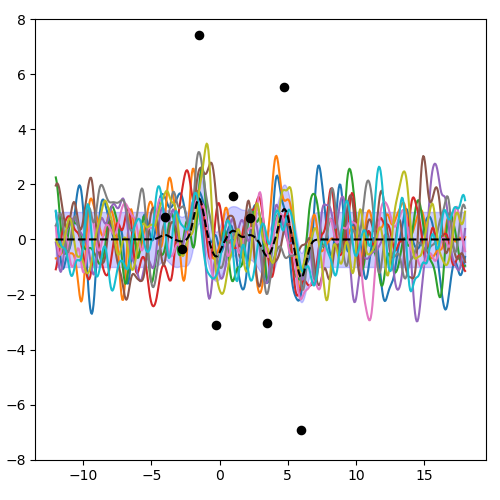
\includegraphics[width=0.4\textwidth]{fig/Q10-post-l050-nvar4.png}
  }
  \vskip\baselineskip
  \subfloat[$l = 1.0$]{%
  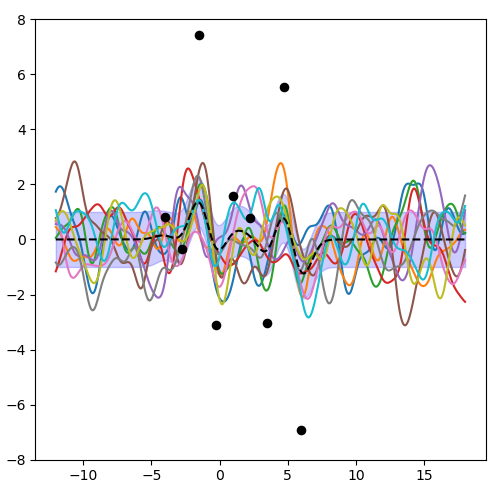
\includegraphics[width=0.4\textwidth]{fig/Q10-post-l100-nvar4.png}
  }
  \hfill
  \subfloat[$l = 10.0$]{%
  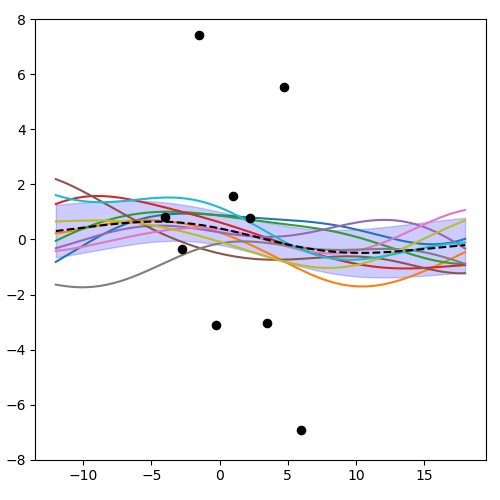
\includegraphics[width=0.4\textwidth]{fig/Q10-post-l1000-nvar4.png}
  }
  \caption{Sample functions, mean and variance of the prediction posterior with 
           different length scales, noise variance = 4}
  \label{fig:Q11-predict-post-noise4}
\end{figure}


\end{question}

\begin{question}{12}
This prior encodes that we have no information about the latent variable $\mathbf{X}$.
Therefore, we assume that it is a zero-mean unit-covariance Gaussian. We do that becasue
we are looking for data to provide more information about the representation transform.
\end{question}

\begin{question}{13}
Consider the linear equation of $\mathbf{Y}(\mathbf{X})$:
\begin{align*}
  \mathbf{Y}(\mathbf{X}) &= \mathbf{W}\mathbf{X} + \mathbf{M} + \mathbf{E} \\
  \mathbf{E} &= [\bm{\epsilon}, \bm{\epsilon}, ..., \bm{\epsilon}] \\
  \mathbf{M} &= [\bm{\mu}, \bm{\mu}, ..., \bm{\mu}] \\  
\end{align*}

And each column of $\mathbf{Y}$ can be written as:
\begin{align*}
  \mathbf{y}_i = \mathbf{W}\mathbf{x}_i + \bm{\mu} +\bm{\epsilon}
\end{align*}
Because $p(\mathbf{X})$ and $p(\mathbf{Y}\mid\mathbf{X}, \mathbf{W})$ are Gaussian, 
 the marginal distribution is also Gaussian.
 Furthermore, we can consider each $\mathbf{y}_i$ are indepenent. Therefore, 
 we can write:
\begin{align*}
  p(\mathbf{Y}\mid\mathbf{W}) &= \prod_{i=1}^{N} p(\mathbf{y}_i\mid\mathbf{W}) \\
  p(\mathbf{y}_i\mid\mathbf{W}) &= N(\mathbf{y}_i\mid \mathbb{E}[\mathbf{y}_i], \text{cov}[\mathbf{y}_i])
\end{align*}
Then, our job is to calculate the mean and covariance of the Gaussian.

Notes that $\mathbf{W}$ is given, $\bm{\epsilon} \sim \mathcal{N}(\mathbf{0}, \sigma^2\mathbf{I})$
 and $\mathbf{x}_i \sim \mathcal{N}(\mathbf{0}, \mathbf{I})$ as 
 $p(\mathbf{X}) = \mathcal{N}(\mathbf{0}, \mathbf{I})$
\begin{align*}
  \mathbb{E}[\mathbf{y}_i] &= \mathbb{E}[\mathbf{W}\mathbf{x}_i + \bm{\epsilon}] \\ 
  &= \mathbb{E}[\mathbf{W}\mathbf{x}_i + \bm{\epsilon}] \\
  &= \bm{\mu} + \mathbf{0} \\
  &= \bm{\mu} \\
  \text{cov}[\mathbf{y}_i] 
  &= \mathbb{E}[(\mathbf{W}\mathbf{x}_i + \bm{\epsilon})
                (\mathbf{W}\mathbf{x}_i + \bm{\epsilon})^{T}] \\
  &= \mathbb{E}[\mathbf{W}\mathbf{x}_i\mathbf{x}_i^T\mathbf{W}^T]
     + \mathbb{E}[\bm{\epsilon}\bm{\epsilon}^{T}]
     && (\text{noise and }\mathbf{W}\mathbf{x}_i\text{ are uncorrelated}) \\
  &= \mathbf{W}\mathbb{E}[\mathbf{x}_i\mathbf{x}_i^T]\mathbf{W}^T + \sigma^2 \mathbf{I}
     && (\bm{\epsilon} \sim N(\mathbf{0}, \sigma^2\mathbf{I})) \\
  &= \mathbf{W}\mathbf{W}^T + \sigma^2\mathbf{I}
     && (\text{cov}[\mathbf{x}_i] = \mathbf{I})
\end{align*}

The marginal distribution is:
\begin{align*}
  p(\mathbf{Y}\mid\mathbf{W}) 
  &= \prod_{i=1}^{N} 
    \mathcal{N}(\mathbf{y}_i\mid\bm{\mu}, \mathbf{C}) \\
  &= \mathcal{N}(\text{vec}(\mathbf{Y})\mid\text{vec}(\mathbf{M}), \mathbf{I}_N\otimes\mathbf{C})
  \numberthis  \label{eq:q13-result}
\end{align*}
where $\mathbf{C}$ is a covariance matrix defined as:
\begin{equation}\label{eq:q13-matC}
  \mathbf{C} = \mathbf{W}\mathbf{W}^T + \sigma^2\mathbf{I}
\end{equation}
\end{question}

\begin{question}{14}
First, let's write down different estimation in log-space.

Consider we have a linear relation $\mathbf{Y}(\mathbf{X})$ mentioned in Question 13
and set $\bm{\mu} = \mathbf{0}$.
\\ 
Maximum-likelihood estimation:
\begin{align*}
  \hat{\mathbf{W}} 
  &= \operatorname{argmin}_{\mathbf{W}}
    [\sum_{i=1}^{N} \| \mathbf{y}_i - \mathbf{W}\mathbf{x}_i\|^2]
\end{align*}
It is equivalent to find the parameter with least square method. More data makes
the computational time longer.

Maximum-a-posteriori (MAP) estimation:
\begin{align*}
  \hat{\mathbf{W}} 
  &= \operatorname{argmin}_{\mathbf{W}}
    [\sum_{i=1}^{N} \| \mathbf{y}_i - \mathbf{W}\mathbf{x}_i\|^2
      + \lambda \textbf{vec}(\textbf{W})^T\textbf{vec}(\textbf{W})]
\end{align*}
MAP approach has an extra regularization term for preventing from overfitting.
We have a degree of freedom to choose the regularizer coefficient.
If we have more data, then regularization term will be less important compared
with the least square error term.

Type-II Maximum-Likelihood:
\begin{align*}
  \hat{\mathbf{W}} 
  &= \operatorname{argmin}_{\mathbf{W}}
    [\sum_{i=1}^{N} \mathbf{y}_i^T \mathbf{C}^{-1}\mathbf{y}_i
      + N\log{|\mathbf{C}|}]
\end{align*}
Type-II maximum likelihood approach does not depends on $\mathbf{X}$ and it is
very useful in our case. $N\log{|\mathbf{C}|}$ expresses the model complexity
and $\sum_{i=1}^{N} \mathbf{y}_i^T \mathbf{C}^{-1}\mathbf{y}_i$ plays the role of
goodness of fit. When data become more, the penalty of the model complexity becomes
more important.
  
The last two expression of Eq. 25 are equivalent. It is because the denominator:
  \begin{align*}
    \int p(\mathbf{Y}\mid\mathbf{X}, \mathbf{W})p(\mathbf{W})d\mathbf{W}
  \end{align*}
is not a function of $\mathbf{W}$. And we know that that integral gives a possitive
real number. Therefore, when finding the maximum value of $\mathbf{W}$, the denominator 
can be ignored.

The Type-II Maximum-likelihood is a sensible approach since it consider how to
 choose a parameter $\mathbf{W}$ which maximizes the model evidence. In other words,
 it is in the sense that we choose a parameter to maximize the probability of 
 getting such a set of observations.
\end{question}


\begin{question}{15}
The course book chapter 12.2.1 has the similar formulation.\\
The objective function:
\begin{align*}
  \mathcal{L}(\mathbf{W}) &= -\log(p(\mathbf{Y}\mid\mathbf{W})) \\
  &= -\prod_{i=1}^{N} \mathcal{N}(\mathbf{y}_i\mid\mathbf{0}, \mathbf{C})
      && \text{(use eq. \eqref{eq:q13-result})} \\
  &= \frac{ND}{2}\log{2\pi} + \frac{N}{2}\log(|\mathbf{C}|) 
     + \frac{1}{2} \sum_{i=1}^{N} (\mathbf{y}_i - \bm{\mu})^T \mathbf{C}^{-1}(\mathbf{y}_i - \bm{\mu}) \\
  &= \frac{N}{2}[D\log(2\pi) + \log(|\mathbf{C}|) + \text{Tr}(\mathbf{C}^{-1}\mathbf{S})]
\end{align*}
where $\mathbf{S}$ is defined as:
\begin{align*}
  \mathbf{S} = \frac{1}{N}\sum_{i=1}^{N} (\mathbf{y}_i - \bar{\mathbf{y}})(\mathbf{y}_i - \bar{\mathbf{y}})^T
\end{align*}
Since $\bm{\mu}$ is estimated as $\bar{\mathbf{y}}$ by maximum likelihood method with respect to $\bm{\mu}$.
We should notice that $\mathbf{S}$ is a symmetric matrix since $\mathbf{S}$ indeed is a data covariance matrix.

Below is the derive of the gradient in element-wise approach. The Matrix cookbook 2012 Ed.
is used in this derive. "cookbook Eq.133" means using the equation 133 in the cookbook.\\
Consider equation \eqref{eq:q13-matC} in element-wise form:

Obviously, we have:
\begin{equation}
  \frac{\partial}{\partial \mathbf{W}}\frac{ND}{2}\log{2\pi} = 0
  \label{eq:Q15-dL0}
\end{equation}
\begin{align*}
  C_{kl} &= (\mathbf{W}\mathbf{W}^T + \sigma^2\mathbf{I})_{kl} \\
  &= \sum_{\theta}(W_{k\theta}W_{l\theta}) + \sigma^2\delta_{kl} \\
  \frac{\partial C_{kl}}{\partial W_{ij}} 
  &= \frac{\partial}{\partial W_{ij}}\sum_{\theta}W_{k\theta}W_{l\theta} \\
  &= \sum_{\theta}[W_{l\theta}\frac{\partial W_{k\theta}}{\partial W_{ij}} 
                 + W_{k\theta}\frac{\partial W_{l\theta}}{\partial W_{ij}}] \\
  &= \sum_{\theta}[W_{l\theta}\delta_{ik}\delta_{\theta j} + W_{k\theta}\delta_{il}\delta_{\theta j}]
    &&(\sum_{\theta}(a_{i\theta}\delta_{\theta j}) = a_{ij}) \\
  &= W_{lj}\delta_{ik} + W_{kj}\delta_{il} \numberthis \label{eq:dCdW}
\end{align*}
Consider the derivatives of $\frac{N}{2}\log(|\mathbf{C}|)$:
\begin{align*}
  \frac{\partial}{\partial W_{ij}}\frac{N}{2}\log(|\mathbf{C}|)
  &= \frac{N}{2}[\sum_{k,l} \frac{\partial \log(|\mathbf{C}|)}{\partial C_{kl}}
                           \frac{\partial C_{kl}}{\partial W_{ij}} ]
      && (\text{cookbook Eq.133}) \\
  &= \frac{N}{2}[\sum_{k,l} ((\mathbf{C}^T)^{-1})_{kl}
                            \frac{\partial C_{kl}}{\partial W_{ij}} ]
      && (\text{cookbook Eq.57}) \\
  &= \frac{N}{2}[\sum_{k,l} (\mathbf{C}^{-1})_{kl}
                 (W_{lj}\delta_{ik} + W_{kj}\delta_{il})]
      && (\text{use eq.\eqref{eq:dCdW} and } \mathbf{C}^T = \mathbf{C}) \\
  &= \frac{N}{2}[\sum_{k,l} (\mathbf{C}^{-1})_{kl}W_{lj}\delta_{ik}
        + \sum_{k,l} (\mathbf{C}^{-1})_{kl}W_{kj}\delta_{il}] \\
  &= \frac{N}{2}[\sum_{l} (\mathbf{C}^{-1})_{il}W_{lj}
        + \sum_{k} (\mathbf{C}^{-1})_{ki}W_{kj}] \\
  &= \frac{N}{2}[\sum_{l} (\mathbf{C}^{-1})_{il}W_{lj}
        + \sum_{k} (\mathbf{C}^{-1})_{ik}W_{kj}]
      && (\mathbf{C}^{-1} = (\mathbf{C}^{-1})^T) \\
  \frac{\partial}{\partial \mathbf{W}}\frac{N}{2}\log(|\mathbf{C}|)
  &= \frac{N}{2}[2\mathbf{C}^{-1}\mathbf{W}] \\
  &= N\mathbf{C}^{-1}\mathbf{W} \numberthis \label{eq:Q15-dL1}
\end{align*}
For the sake of convenience, we define $\mathbf{C}^{-T} = (\mathbf{C}^{-1})^T$.
Obviously, we have:
\begin{align*}
  \mathbf{C}^{-T} &= (\mathbf{C}^{-1})^T \\
                  &= (\mathbf{C}^{T})^{-1} \\
  \mathbf{C}^{-T} &= \mathbf{C}^{-1} \numberthis \label{eq:C^-T}
\end{align*}
Consider the derivatives of $\frac{N}{2}\text{Tr}(\mathbf{C}^{-1}\mathbf{S})$:

\begin{align*}
  \frac{\partial}{\partial W_{ij}}&\frac{N}{2}\text{Tr}(\mathbf{C}^{-1}\mathbf{S}) \\
  &= \frac{N}{2}[\sum_{k,l} \frac{\partial \text{Tr}(\mathbf{C}^{-1}\mathbf{S})}{\partial C_{kl}}
                            \frac{\partial C_{kl}}{\partial W_{ij}} ]\\
  &= \frac{N}{2}[\sum_{k,l} (-\mathbf{C}^{-T}\mathbf{S}^{T}\mathbf{C}^{-T})_{kl}
                            \frac{\partial C_{kl}}{\partial W_{ij}} ]\\
  &= -\frac{N}{2}[\sum_{k,l} (\mathbf{C}^{-1}\mathbf{S}^{T}\mathbf{C}^{-1})_{kl}
                            (W_{lj}\delta_{ik} + W_{kj}\delta_{il}) ]       
      &&(\text{use eq.\eqref{eq:dCdW} and \eqref{eq:C^-T}})  \\
  &= -\frac{N}{2}[\sum_{l} (\mathbf{C}^{-1}\mathbf{S}\mathbf{C}^{-1})_{il}W_{lj}
                + \sum_{k} (\mathbf{C}^{-1}\mathbf{S}\mathbf{C}^{-1})_{ki}W_{kj}] 
      &&(\mathbf{S}^T = \mathbf{S})  \\
  &= -\frac{N}{2}[\sum_{l} (\mathbf{C}^{-1}\mathbf{S}\mathbf{C}^{-1})_{il}W_{lj}
                + \sum_{k} (\mathbf{C}^{-1}\mathbf{S}\mathbf{C}^{-1})_{ik}W_{kj}]
      &&(\text{See eq.}\eqref{eq:CSC_sym})  \\
\end{align*}

In matrix form, we have:
\begin{equation}
  \frac{\partial}{\partial \mathbf{W}}\frac{N}{2}\text{Tr}(\mathbf{C}^{-1}\mathbf{S})
  = -N\mathbf{C}^{-1}\mathbf{S}\mathbf{C}^{-1}\mathbf{W}
  \label{eq:Q15-dL2}
\end{equation}

$\mathbf{C}^{-1}\mathbf{S}\mathbf{C}^{-1}$ is a symmetric matrix since:
\begin{align*}
  (\mathbf{C}^{-1}\mathbf{S}\mathbf{C}^{-1})^{T} 
  &= \mathbf{C}^{-T}\mathbf{S}^T\mathbf{C}^{-T} \\
  &= \mathbf{C}^{-1}\mathbf{S}\mathbf{C}^{-1}
  \numberthis \label{eq:CSC_sym}
\end{align*}


Combine eq. \eqref{eq:Q15-dL0}, \eqref{eq:Q15-dL1} and \eqref{eq:Q15-dL2} we have:
\begin{align*}
  \frac{\partial{\mathcal{L}}}{\partial{\mathbf{W}}} 
    &= N(\mathbf{C}^{-1}\mathbf{W} 
         - \mathbf{C}^{-1}\mathbf{S}\mathbf{C}^{-1}\mathbf{W})
\end{align*}
\end{question}

\begin{question}{16}
Figure \ref{fig:q16-replearn} shows both the learned and the origal 
representation of $\mathbf{x}$.
The representation is generated from the mapping $f_{non-lin}$.

We can see that there is a rotational symmetry between the learned representation
and the original representation. It is becasue we have a degree of freedom to choose
a $\widetilde{\mathbf{W}}$ which is related to rotate the latent space coordinates.

Consider $\widetilde{\mathbf{W}} = \mathbf{WR}$. In the linear model 
$\mathbf{Y}(\mathbf{X}) = \mathbf{WX} + \bm{\mu} + \bm{\epsilon}$, 
$\mathbf{R}$ can be considered as rotating the coordinates of the 
latent variable space.

In our objective function $\mathcal{L}(\mathbf{W})$, it is invariant if we chossing
a $\widetilde{\mathbf{W}}$ which satisfies the relation $\widetilde{\mathbf{W}} = \mathbf{WR}$.
  \begin{align*}
    \mathbf{C}(\widetilde{\mathbf{W}}) 
      &= \widetilde{\mathbf{W}}\widetilde{\mathbf{W}}^T + \sigma^2\mathbf{I} \\
      &= \mathbf{W}\mathbf{R}\mathbf{R}^T\mathbf{W}^T + \sigma^2\mathbf{I} \\
      &= \mathbf{W}\mathbf{W}^T + \sigma^2\mathbf{I}
        && (\mathbf{R}\mathbf{R}^T = \mathbf{I}) \\
      &= \mathbf{C}(\mathbf{W})
  \end{align*}
$\mathbf{R}\mathbf{R}^T = \mathbf{I}$ since $\mathbf{R}$ is a rotation matrix.
And we also have:
  \begin{align*}
    \mathcal{L}(\widetilde{\mathbf{W}})
      &= \frac{N}{2}[D\log(2\pi) 
        + \log(|\mathbf{C}(\widetilde{\mathbf{W}})|) 
        + \text{Tr}(\mathbf{C}(\widetilde{\mathbf{W}})^{-1}\mathbf{S})] \\
      &= \frac{N}{2}[D\log(2\pi) 
        + \log(|\mathbf{C}(\mathbf{W})|) 
        + \text{Tr}(\mathbf{C}(\mathbf{W})^{-1}\mathbf{S})]
        && (\mathbf{C}(\widetilde{\mathbf{W}}) = \mathbf{C}(\mathbf{W})) \\
      &= \mathcal{L}(\mathbf{W})
  \end{align*}

Therefore, the objective function and the corresponding marginal likelihood
$p(\mathbf{Y}\mid\mathbf{W})$
are invariant with respect to chossing a $\widetilde{\mathbf{W}}$ which satisfies
$\widetilde{\mathbf{W}} = \mathbf{WR}$.

The scale of the learned representation is magnified for easier comparsion.
\begin{figure}[h!]
  \centering
  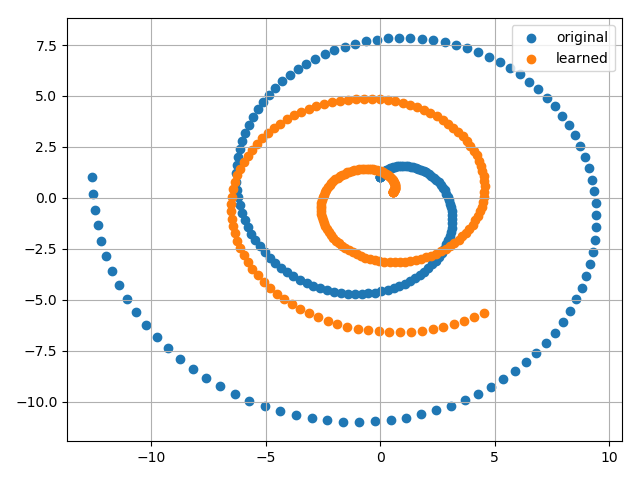
\includegraphics[width=0.5\linewidth]{fig/Q16-replearn.png}
  \caption{Plot learned and original representations of $\mathbf{X}$}
  \label{fig:q16-replearn}
\end{figure}
\end{question}

\begin{question}{17}
It is the simplest model since it has zero degree of freedom to change the model.
The model implies that there is a equal probability of generating different kinds of
data. To answer whether a model is good bad model, it depends the evidence
of the data. 

In the figure \ref{fig:q17-model-evidence}, $M_1$ is a good model and $M_0$ is a 
bad model to $\mathcal{D}_1$ according both Occam’s Razor rule and the probability
of evidence. However, to $\mathcal{D}_2$, $M_1$ is a bad model since $M_1$ places
zero probability over $\mathcal{D}_2$ and $M_0$ becomes a good model to $\mathcal{D}_2$.
\begin{figure}[h!] %TODO: fix the figure. model1 -> model 100
  \centering
  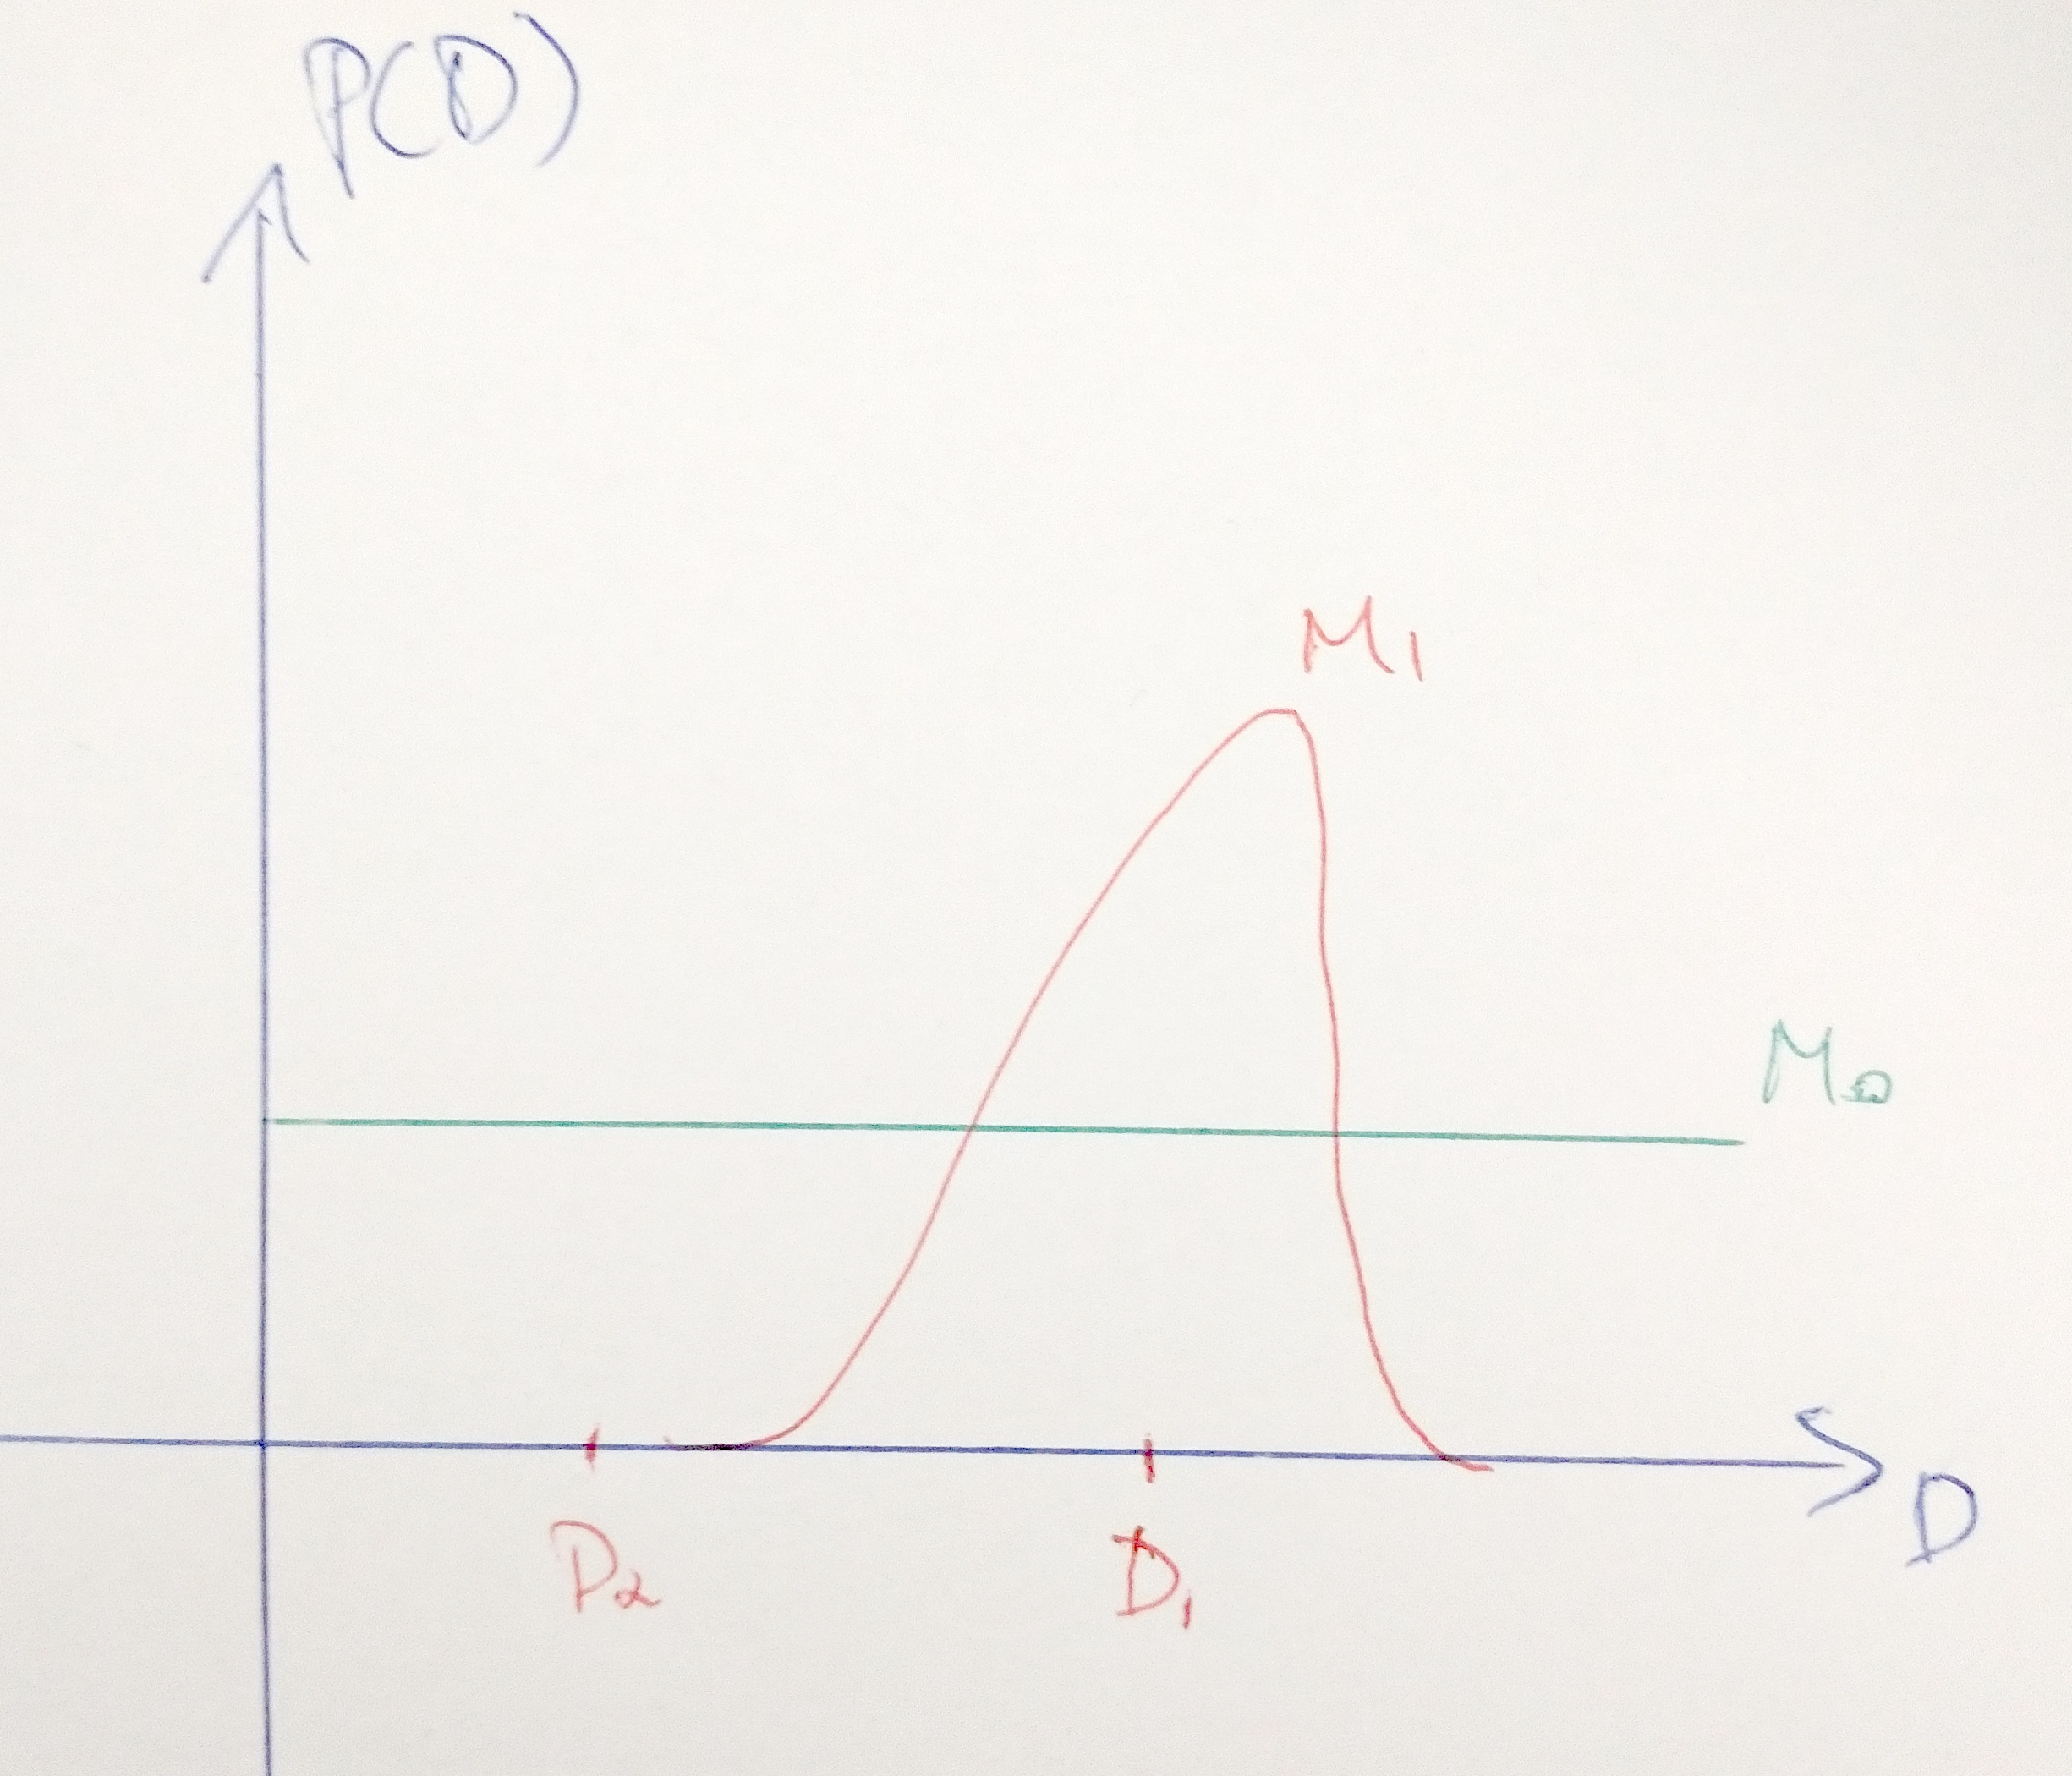
\includegraphics[width=0.5\linewidth]{fig/Q17.jpg}
  \caption{The probability of evidence of each model}
  \label{fig:q17-model-evidence}
\end{figure}
\end{question}

\begin{question}{18}
Each model is the probability of the outcome $t^i$ given the model and model
parameters:
\begin{align*}
  p(t^n\mid M_1, \bm{\theta}_1) = \frac{1}{1 + \exp(-t^n\theta^1_1 x^n_1)}
\end{align*}
This is a logistic regression. Since for each model, we can treat it as a 
two-class classification problem. That is giving a grid location as input, 
predict the output $t^i$ which is either 1 or -1.

Model $M_1$ is more flexible compared to $M_0$ since $M_1$ has one 
free parameter. It is the weighting of $x^n_1$ and $x^n_1$ is one of the coordinate
of the grid.

Since $M_1$ consider only one coordinate of the grid, we can imagine that only a 
small subset of data can be captured by this model. 
For example, If $x^n_1$ represents the column index of the grid, then only whole
column has the same output can be explained by this model.
Therefore, the model $M_1$ has a small spreading of its probability mass over 
$\mathcal{D}$.
\end{question}

\begin{question}{19}
The terms in the exponent of the logistic equation can be considered as 
a linear speration plane.
$M_2$ and $M_3$ are considered as more flexible linear speration planes on the grid.
Choosing the form of $M_1$, $M_2$, and $M_3$, we only choose linear separable data.
Therefore, $M_1$, $M_2$, and $M_3$ place probability mass over the linear separable
dataset.

The linear separable datasets are suitable for the models $M_1, M_2, M_3$.

To the number of data sets each model can explain, $M_3$ is the most, then followed
by $M_2$, and then $M_1$.
The uncertainty of models can be considered as ($1 - p(d_i\mid M_i)$),
where $d_i$ is one of the data sets.
Since the sum of probability over a random variable space must be one. The more
data sets a model can explain, the less certainty (i.e. $p(d_i\mid M_i)$)
the model can have.

In terms of number of model parameters, $M_3$ is more flexible then $M_2$ since
$M_3$ has three parameters and $M_2$ has two.
In addition, $M_3$ can be considered as realization of other models 
${M_1, M_2}$ by setting some parameters to zero.
Therefore, $M_3$ is the most flexible among those four models.
On the other hand, $M_0$ are considered as the most restrictive since
it have no model parameter.

In terms of the number of data set a model can explain, $M_0$ is the most
flexible since it can explain all possible data by the uniform probability 
distribution.
$M_3$ is more flexible than $M_2$ and $M_1$. $M_2$ can explain data which can 
also be explained by $M_3$ except one situation. That situation is all
grid are of the same output. It is because of the bias term $\theta^3_3$.
\end{question}

\begin{question}{20}
In marginalization, we can encode our beliefs by setting the prior on a variable.
The variable usually we are not interested in our model.

The implication of the process is to calculate the weighted average of the model
likelihood according the prior on the parameters.

The evidence can also be regarded as the probability of generating the data set 
$\mathcal{D}$ from a model describled by all possible parameters. That is 
the reason why we average the likelihood weighted by the probability of each parameter.
\end{question}

\begin{question}{21}
First, the spherical Gaussian prior implies that all components of the weighting
vector $\bm{\theta}$ are indepenent.

Second, large variance of the weighting factor allows to sample a weighting vector
with large L2-norm from the distribution. 
In the sense of SVM, the margin of the sparation plain is 
inversely proportional to the L2-norm of the weighting vector. Therefore, we
allow the speration plane with a large uncertainty and high 
flexiblity.
\end{question}

\begin{question}{22}
The sum of the evidence over all data sets which belong to $\mathcal{D}$ is 1. 
It means given a model $M_i$ sum the probability over all possible data sets 
and it obviously equals to 1. It also means that each
$p(\mathcal{D}\mid M_i)$ is a valid probability distribution.

The evidence over the whole dataset is shown in figure \ref{fig:PlotEvid}.

Take a look on figure \ref{subfig-2:plotEvidSub}.
Considering the spreading of probability mass of each model, we can find that
$M_0$ spreads its probability mass over whole region of data set. And the dataset
region covered by $M_3$ is greater than $M_2$ and the data set region of $M_2$ 
is greater than $M_1$.

We can consider the parameterization scheme employed by each model. 
$M_1$ represents
a vertical speration plane (if we consider $x_0$ as the column index of the grid).
The model is simple enough so that the amount of data set can be explained by this
model is limited. 
$M_2$ can be viewed as a speration plane passing through the origin and $M_2$ is then 
flexible than $M_1$. Thus the region covered by $M_2$ is larger by $M_1$.
$M_3$ is more flexible since it is a speration plane allowed to have offset from the
origin. Hence, $M_3$ can explain all linear speratable data.

\begin{figure}[h]
  \subfloat[Plot evident against all data sets, $\mathcal{D}$\label{subfig-1:plotEvidAll}]{%
  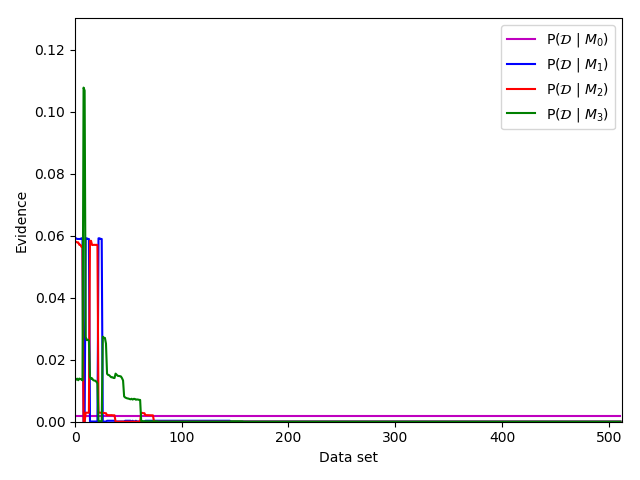
\includegraphics[width=0.45\textwidth]{fig/Q22-all.png}
  }
  \hfill
  \subfloat[Plot evident against possible data sets, $\mathcal{D}$\label{subfig-2:plotEvidSub}]{%
  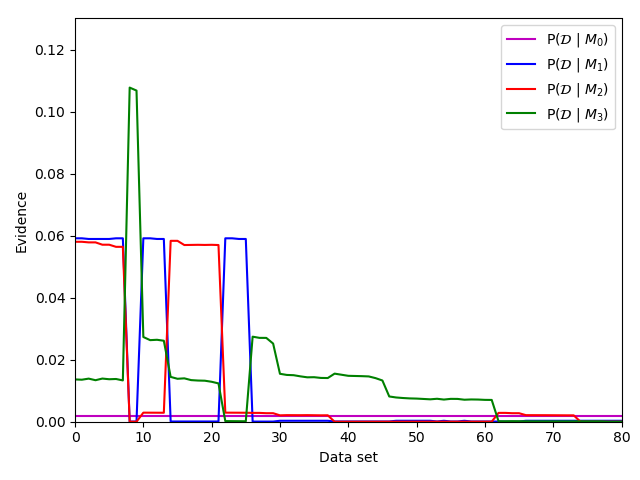
\includegraphics[width=0.45\textwidth]{fig/Q22-sub.png}
  }
  \caption{Plot evidence against all data set $\mathcal{D}$ for different models}
  \label{fig:PlotEvid}
\end{figure}
\end{question}

%TODO: review Q23
\begin{question}{23}
\begin{table}[h]
    \centering
    \subfloat[Highest evidence data set]{%
      \hspace{2cm}%
      \begin{tabular}{|c|c|c|} 
        \hline
        X & X & O \\
        \hline
        X & O & O \\
        \hline
        X & O & O \\
        \hline
      \end{tabular}\label{subtable:M1-high}
      \hspace{2cm}%
    }\hspace{1cm}
    \subfloat[Lowest evidence data set]{%
      \hspace{2cm}%
      \begin{tabular}{|c|c|c|}
        \hline
        X & O & O \\
        \hline
        O & X & X \\
        \hline
        O & O & O \\
        \hline
      \end{tabular}\label{subtable:M1-low}
      \hspace{2cm}%
    }
  \caption{The highest and lowest evident data set for $M_1$}
  \label{table:M1}
\end{table}
Since $M_1$ can be considered as a vectical seperation plane passing through the
origin, it is sensible to see such configuration in table
(\ref{subtable:M1-high}).
In table (\ref{subtable:M1-low}), we can see that it is not possible to draw any
vertical line to seperate crosses and circles.

\begin{table}[h]
  \centering
  \subfloat[Highest evidence data set]{%
    \hspace{2cm}%
    \begin{tabular}{|c|c|c|} 
      \hline
      X & X & O \\
      \hline
      X & O & O \\
      \hline
      X & O & O \\
      \hline
    \end{tabular}\label{subtable:M2-high}
    \hspace{2cm}%
  }\hspace{1cm}
  \subfloat[Lowest evidence data set]{%
    \hspace{2cm}%
    \begin{tabular}{|c|c|c|}
      \hline
      O & X & O \\
      \hline
      X & O & X \\
      \hline
      O & X & O \\
      \hline
    \end{tabular}\label{subtable:M2-low}
    \hspace{2cm}%
  }
  \caption{The highest and lowest evident data set for $M_2$}
\label{table:M2}
\end{table}
For $M_2$, it is a speration line restricted to pass through the origin the 
center of the grid.
It is possible to use a left-bottom to up-right diagonal line to sperate crosses
and circles as shown in table (\ref{subtable:M2-high}). While it is not possible 
to use any line passing through the middle box to sperate crosses and circles in
table (\ref{subtable:M2-low}).

\begin{table}[h]
  \centering
  \subfloat[Highest evidence data set]{%
    \hspace{2cm}%
    \begin{tabular}{|c|c|c|} 
      \hline
      X & X & X \\
      \hline
      X & X & X \\
      \hline
      X & X & X \\
      \hline
    \end{tabular}\label{subtable:M3-high}
    \hspace{2cm}%
  }\hspace{1cm}
  \subfloat[Lowest evidence data set]{%
    \hspace{2cm}%
    \begin{tabular}{|c|c|c|}
      \hline
      O & X & O \\
      \hline
      X & X & X \\
      \hline
      X & O & O \\
      \hline
    \end{tabular}\label{subtable:M3-low}
    \hspace{2cm}%
  }
  \caption{The highest and lowest evident data set for $M_3$}
\label{table:M3}
\end{table}

It is noted that $M_3$ is the only model having a bias term (interception term)
in the logistic regression term. 
$M_3$ is the only model can explain all circles and crosses
cases with its bias term. Moreover, the prior has the preference on chossing large
parameters with its large variance. Therefore, the prior makes the seperate line 
to have a large intercept and the line most likely seperate the data shown in table 
(\ref{subtable:M3-high}).
The peak of $M_3$ in 
figure \ref{subfig-2:plotEvidSub} can also be explained by all circles and all crosses. 
Therefore, the model evidence of all circles or crosses is the highest for $M_3$.

The data set shown in table(\ref{subtable:M3-low}) is not linear separable.
\end{question}

\begin{question}{24}
The effect of the prior $p(\theta)$ controls what parameters we can sample from it.

Consider $M_0$ can be writen as:
\begin{align*}
  p(\mathcal{D} \mid M_0, \bm{\theta}_0) &= \frac{1}{2^9} \\
    &= \prod_{n=0}^{9}\frac{1}{1 + \exp(0)}
\end{align*}

If we use a extreme small $\sigma^2$, says $\sigma^2 = 10^{-6}$, we would probably
sample all zeros from it. Therefore, all model will reduce to $M_0$.
If we use a very large $\sigma^2$, says $\sigma^2 = 10^{6}$, we would probably
arbitrary large number from the prior. However, the seperation line slope depends
on the ratio of two of the parameters. Therefore, the evidence plot would not change
as in our previous case.

If we use a non-diagonal covariance matrix for the prior, we somehow impose
contrains over parameters. The marginalisation carries the this information to 
the model evidence $p(\mathcal{D}\mid M_i)$. Therefore, we can consider
that the models $\{{M_i}\}_{i=1}^3$ becomes restrictive under dependent choice 
of parameter compared to indepenent choice. Each model covers smaller amount of 
data set as show in figure \ref{fig:Q24-non-diag-plotEvid}.
\begin{figure}[h] 
  \centering
  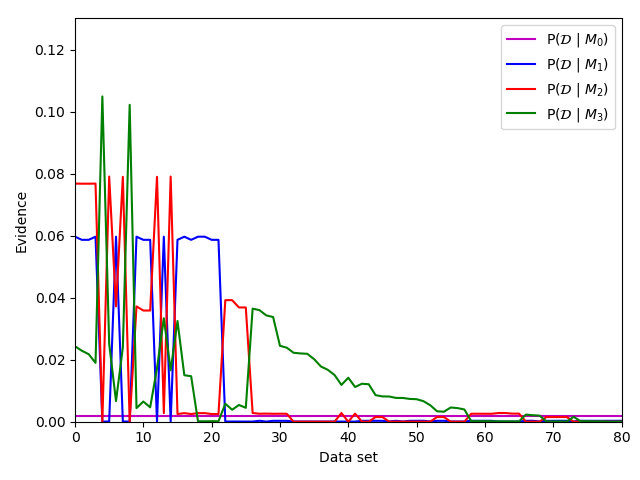
\includegraphics[width=0.5\linewidth]{fig/Q24-non-diag.png}
  \caption{Plot evidence against data set with a non-diagonal parameter prior}
  \label{fig:Q24-non-diag-plotEvid}
\end{figure}

If we use a non-zero mean prior such as $\mu = [5, 5, 5]^T$, we can see that
some model favor on specific data sets. It is because there are peaks in figure
\ref{fig:Q24-non-zero-plotEvid}. Those data sets are diagonal separable since 
we make a perference on the choice of parameter.

The region covered by each model should be almost the same as the zero-mean prior.
It is because the flexiblity of models holds when changing the mean of prior.
  
  \begin{figure}[h] 
    \centering
    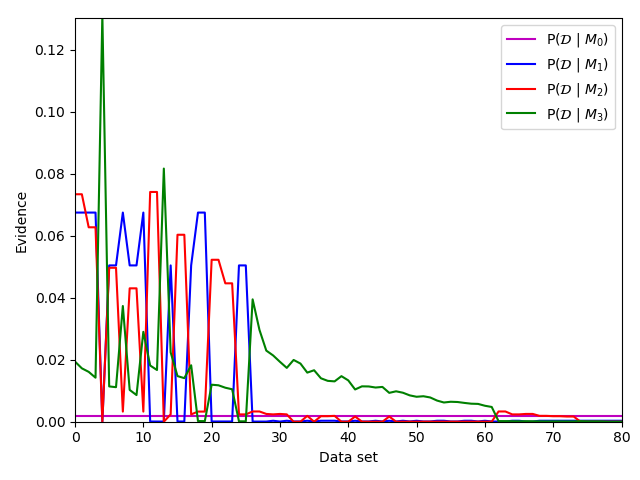
\includegraphics[width=0.5\linewidth]{fig/Q24-non-zero-mean-sub.png}
    \caption{Plot evidence against data set with a non-zero mean parameter prior}
    \label{fig:Q24-non-zero-plotEvid}
  \end{figure}
\end{question}
% --------------------------------------------------------------
\end{document}
